 \documentclass[12pt]{article}

\usepackage{dcolumn}
\usepackage{booktabs}
\usepackage{pdflscape}
\usepackage{graphicx}
\usepackage{placeins}
\usepackage{amsmath}
\usepackage{hyperref}
\usepackage[title]{appendix}
\usepackage[margin = 3cm]{geometry}
\linespread{1.5}
\usepackage{xepersian}
\settextfont{XB Zar}
\setdigitfont{XB Zar}

\begin{document}
\title{دامنه نوسان}
\author{سید مرتضی آقاجان‌زاده}
\maketitle

برخلاف اکثر بازار های مالی دنیا در بازار بورس اوراق بهادار تهران براساس ویژگی‌های نماد، محدودیت‌ روزانه نوسان  وجود دارد و با توجه به این دامنه در این بازار، استراتژی‌های خرید و فروش متنوعی شکل گرفته‌است. 
آیا برخورد قیمت به این محدودیت روزانه، سبب جلب توجه سرمایه‌گذاران می‌شود و در بازده و حجم روزانه سهم تغییر ایجاد می‌کند؟ 


در بازار‌های مالی به طور معمول تعداد قابل توجهی نماد در حال معامله می‌باشد. این تنوع نماد سبب می‌شود تا سرمایه‌گذاران در هنگام تصمیم‌گیری برای خرید و فروش با مجموعه انتخاب‌های گوناگونی مواجه باشند. از طرفی سرمایه‌گذاران توانایی و توجه کافی جهت بررسی تمامی نماد‌های موجود در بازار را ندارند.
از این رو سرمایه‌گذاران هنگام تصمیم‌گیری در رابطه با خرید و فروش نماد با جست‌و‌جو‌‌ای دشوار مواجه هستند. 
در این فضا هر اتفاقی که سبب جلب توجه سایرین به نماد گردد می‌تواند در راستای محدود کردن مجوعه بررسی سرمایه‌گذاران کمک کننده باشد.
در این زمینه پیش‌بینی می‌شود در حضور اتفاقاتی که سبب جلب توجه به نماد می‌شود حجمم معاملات و بازده سهم افزایش قابل توجهی پیدا می‌کند و این اتفاق را ناشی از اخبار منتشر نشده از نماد تلقی می‌کنند.
 


\section{مطالعات گذشته}
\subsection{\lr{JEF-2007-Seasholes, M. S., \& Wu, G.-Predictable behavior, profits, and attention}}
\label{s1.1}
این مقاله در صدد آن است در بازار سهام شانگهای در روزی که قیمت سهم به حد بالایی محدوده قیمتی برخورد می‌کند از خود بازده بالا، حجم بالا و پوشش خبری نشان می‌دهد. این اتفاق توجه سرمایه گذاران را جلب می‌کند. در بازار تعداد سهام بالایی وجود دارد و این اتفاق می‌تواند مجموعه تصمیم گیری سرمایه‌گذاران را محدود کند.این مقاله از داده‌های معاملات روزانه نماد در بازار، قیمت سهام و کلیه معاملات افراد در شهری خاص استفاده کرده‌است تا علاوه بر بررسی حجم معاملات بررسی کند که آیا سرمایه گذاران جدیدی با برخورد قیمت به حد نوسان به سهم جذب می‌شوند یا خیر.


جهت بررسی رفتار سرمایه‌گذاران حقیقی شاخص عدم توازن خالص خرید برای زمان $ t $ و $ t+1 $ را به صورت زیر تعریف می‌کند

\lr{\begin{equation}
\text{Imbalance}_{k,t}^{\text{Indiv}} = \frac{\text{Buys}_{k,t}^{\text{Indiv}} - \text{Sells}_{k,t}^{\text{Indiv}}}{\text{Buys}_{k,t}^{\text{Indiv}} + \text{Sells}_{k,t}^{\text{Indiv}}}
\label{e1}
\end{equation}}
و بیان می‌کند چنانچه برخورد قیمت به حد نوسان توجه سرمایه‌گذاران حقیقی را جذب می‌کند آنگاه این شاخص در دوره $ t+1 $ مثبت است.

از طرفی جهت بررسی حجم معاملات از ملاک‌های زیر استفاده می‌کند که طبعا مانند حال قبل، نیاز است این شاخص‌ها در روزی که قیمت به حد نوسان برخورد می‌کند مثبت باشند.


\lr{\begin{equation}
\text{Turn}_{k,t} = \frac{\text{Volume}(\text{RBM})_{k,t}}{\text{MarketCap(FreeFloat)}_{k,t}}
\label{e2}
\end{equation}}
\lr{\begin{equation}
\text{RelTurn}_{k,t} = \frac{\text{Turn}_{k,t}}{AVG(\text{Turn}_{k,t})}
\label{e3}
\end{equation}}

\begin{figure}[htbp]
\centering
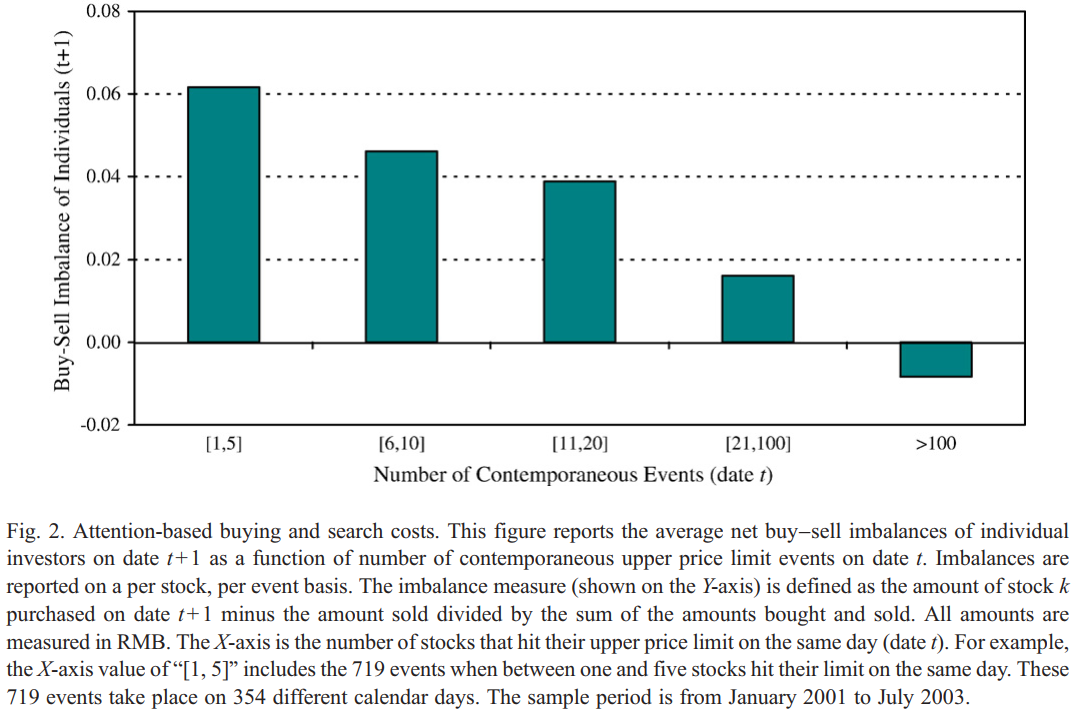
\includegraphics[width=\columnwidth]{g1.png}
\end{figure}
\FloatBarrier
\begin{figure}[htbp]
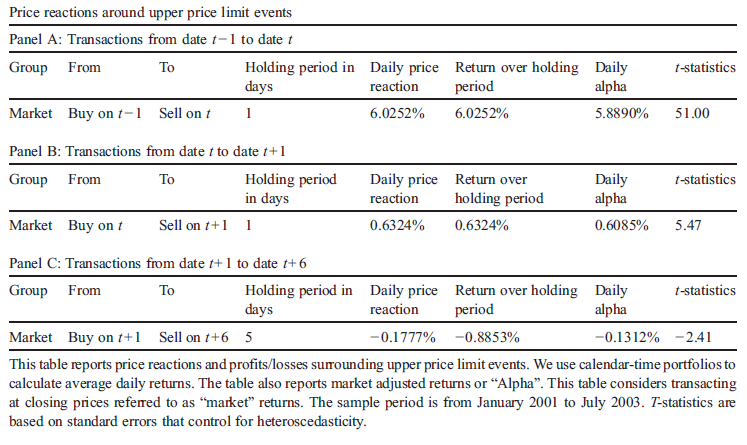
\includegraphics[width=\columnwidth]{Table4.png}
\caption{ نتایج  در مقاله بخش \ref {s1.1}}
\label{g2}
\end{figure}
\FloatBarrier
\subsection{\lr{JE-2019-Ting Chen, Zhenyu Gao, Jibao He, Wenxi Jiang, and Wei Xiong-Daily Price Limits and Destructive Market Behavior}}
\label{s1.2}
در این مقاله در ابتدا بازده سهام در حوالی برخورد قیمت به دامنه نوسان بررسی شده‌است و پس از آن رفتار گونه‌های متفاوت سرمایه‌گذار مورد بررسی قرار گرفته است. در این مقاله از داده‌های در سطح حساب کاربری استفاده شده است.

این مقاله برای بررسی رفتار بازده سهام، از بازده‌های متفاوتی استفاده کرده‌است که در جدول 
\ref{t1} 
به صورت خلاصه بیان شده‌است. منظور از زمان $ t $ روزی است که اتفاق رخ می‌دهد. نتایج برآورد‌ها نیز در شکل
\ref{g1}
بیان شده‌است.
\begin{table}[htbp]
\centering
\begin{tabular}{|r|l|}
\hline
 توضیحات & متغیر\\
\hline

بازده قیمت پایانی نسبت به اولین قیمت در روز $ t $ & 
\lr{Close to open} \\

بازده اولین قیمت در روز $ t+1 $ نسبت به قیمت پایانی در روز $ t $ & 
\lr{Open to close} \\

بازده $ m $ روزه سهام & 
\lr{Day m } \\

بازده تجمعیی بین بازه $ m $ تا $ n $ روز بعد از دوره $ t $ & 
\lr{[m,n] } \\
\hline
\end{tabular}
\caption{خلاصه متغیر‌های وابسته تعریف شده در مقاله بخش \ref{s1.2}}
\label{t1}
\end{table}
کار دیگر مقاله بررسی رفتار سرمایه‌گذاران بزرگ در دوره t و t+1 می‌باشد که با توجه به دسترسی به داده‌های در سطح حساب کاربری این کار امکان پذیر بوده‌است.
نتایج در شکل 
\ref{g3}
نشان داده شده‌است.
\begin{figure}[htbp]
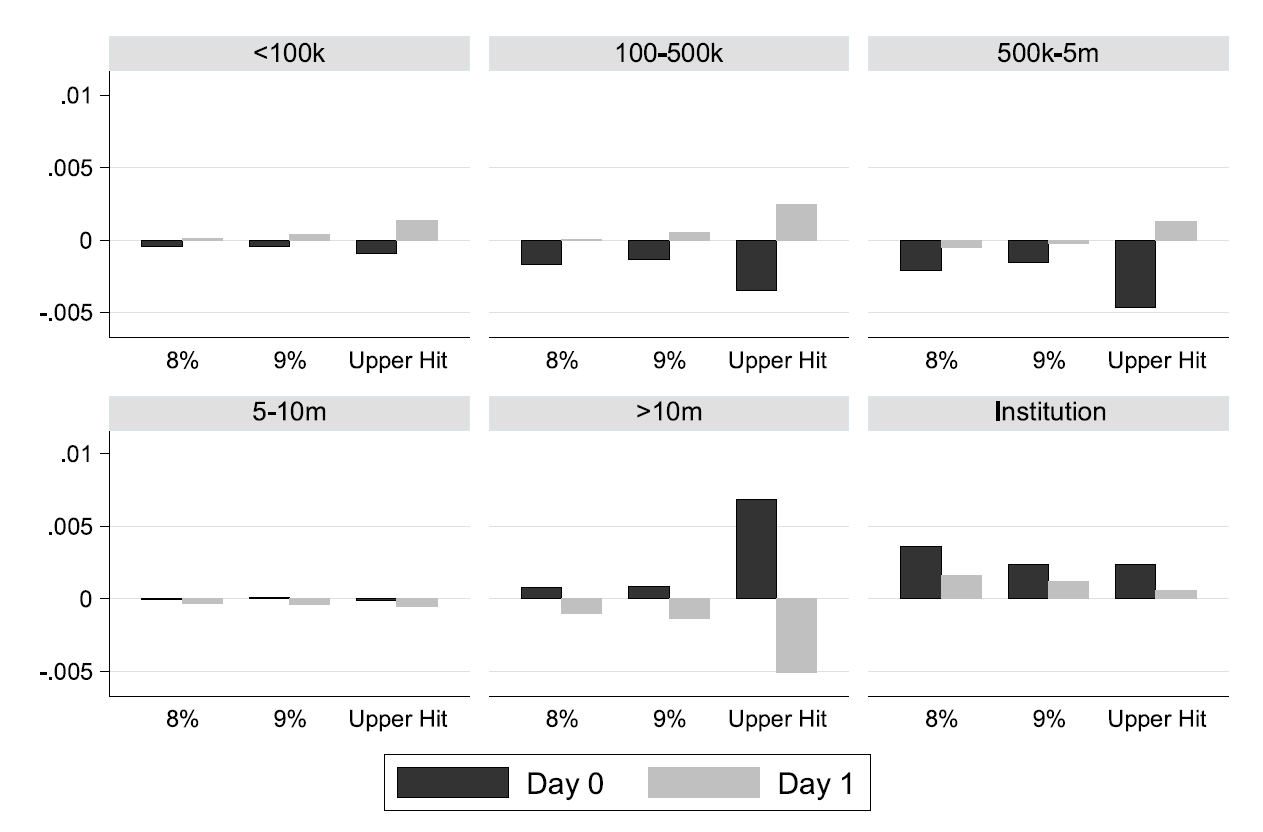
\includegraphics[width=1\columnwidth]{g2.png}
\caption{نتایج بررسی رفتار سرمایه‌گذاران عمده در مقاله بخش \ref {s1.2}}
\label{g3}
\end{figure}

\begin{landscape}
\begin{figure}[htbp]
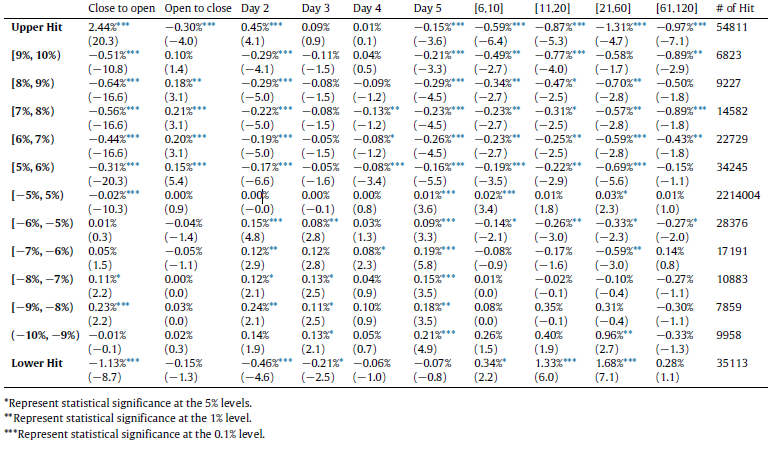
\includegraphics[width=1\columnwidth]{Table1.png}
\caption{خروجی نتایج رگرسیون در مقاله بخش \ref {s1.2}}
\label{g1}
\end{figure}
\end{landscape}
\FloatBarrier


\section{نتایج مقاله با استفاده از داده‌های ایران}
در این قسمت از داده‌های دامنه نوسان روزانه در قسمت سابقه سایت 
\lr{TSETMC}
از ابتدای سال 1396 تا 1399/07/12 استفاده شده‌است.
در بازار سهام ایران انواع مختلف دامنه نوسان از جمله 3،5 و 10 درصد  وجود دارد که در این پژوهش با توجه به آنکه تعداد قابل توجهی از نماد‌ها دارای دامنه نوسان 5 درصد می‌باشند از این نماد‌ها استفاده شده‌است.
 در این بازه برای نماد‌های مورد بررسی، 22044 بار حداکثر قیمت معاملات به سقف دامنه و 16394 بار حداقل قیمت معاملات به کف دامنه برخورد داشته‌است. 
در این بازه به صورت متوسط برای هر نماد 9 روز از 100 روز معاملاتی، قیمت به سقف و 6 روز از 100 روز به کف برخورد داشته‌است. 
خلاصه آماری و توزیع احتمال‌های فوق و دیگر احتمال‌های شرطی در جدول 
\ref{t2}
آورده شده‌است.
با توجه به این جدول احتمال برخورد به سقف دامنه به شرط آنکه در روز قبل قیمت به این سقف برخورد کرده باشد حدودا 
$ 43\% $
می‌باشد. این درصد برای برخورد متوالی قیمت به کف دامنه برابر 
$ 34 \% $
می‌باشد.


{\begin{table}[htbp]
  \centering
 \lr{ \begin{LTR}
    \begin{tabular}{l|c|cc|ccccc}
    Event & {count} & {mean} &{std} &{min} & 25\%  & 50\%  & 75\%  & {max} \\
    \hline
upperHit & 423   & 9.07  & 6.58  & 0     & 4.64  & 8.18  & 11.63 & 54.63 \\
    lowerHit & 423   & 6.55  & 4.68  & 0     & 3.21  & 5.78  & 8.95  & 43.69 \\ 
     u|u   & 422   & 42.99 & 15.16 & 0     & 33.33 & 44.12 & 51.59 & 94.44 \\
     l|u   & 422   & 10.81 & 7.34  & 0     & 6.58  & 10.38 & 14.74 & 94.44 \\
     u|l   & 420   & 14.67 & 9.12  & 0     & 8.39  & 14.29 & 20    & 91.89 \\
     l|l   & 420   & 34.05 & 14.15 & 0     & 25    & 34.25 & 42.55 & 91.89 \\
     u|(u|u) & 415   & 5.09  & 5.25  & 0     & 1.95  & 4.22  & 6.63  & 47.50 \\
     u|(l|l) & 408   & 1.34  & 1.34  & 0     & 0.47  & 1.06  & 1.84  & 12.05 \\
     l|(u|u) & 415   & 1.35  & 1.29  & 0     & 0.50  & 1.09  & 1.92  & 11.73 \\
          l|(l|l) & 408   & 3.08  & 3.17  & 0     & 0.90  & 2.47  & 4.35  & 33.70 \\
    \end{tabular}%}
    \end{LTR}}
      \caption{خلاصه آماری احتمال برخورد قیمت به سقف و کف دامنه نوسان  در سطح نماد}
      \label{t2}
\end{table}}

با توجه به توضیحات مطرح شده در مقدمه، جلب سرمایه‌گذاران به نماد که با برخورد قیمت به سقف یا کف دامنه اتفاق می‌افتد می‌تواند در رفتار بازده، حجم و خرید و فروش حقیقی تغییر ایجاد کند. در نمودار 
\ref{g4}
و
\ref{g5}
ارزش نماد 15 دوره قبل و بعد از برخورد به دامنه نوسان رسم شده‌است. در این دو نمودار به ترتیب ارزش نماد به وسیله بازده روزانه و بازده اضافی نسبت به بازار رسم شده‌است. در این دو نمودار فرض شده‌است ارزش نماد در دوره صفر (دوره برخورد قیمت به دامنه نوسان) برابر یک می‌باشد. همانطور که در این دو نمودار مشاهده می‌شود حادثه برخورد به دامنه نوسان سبب جا‌به‌جایی روند ارزش نماد خواهد‌شد. همانطور که انتظار می‌رفت در نمودار
\ref{g5}
که ارزش نماد به وسیله بازده اضافی نسبت به بازار رسم شده‌است اختلاف روند اندازه بزرگتری دارد که به این معناست برخورد به دامنه نوسان می‌تواند بازده روزانه نماد نسبت به بازار را نیز تحت الشعاع قرار دهد. 
 
\begin{figure}[htbp]
\centering
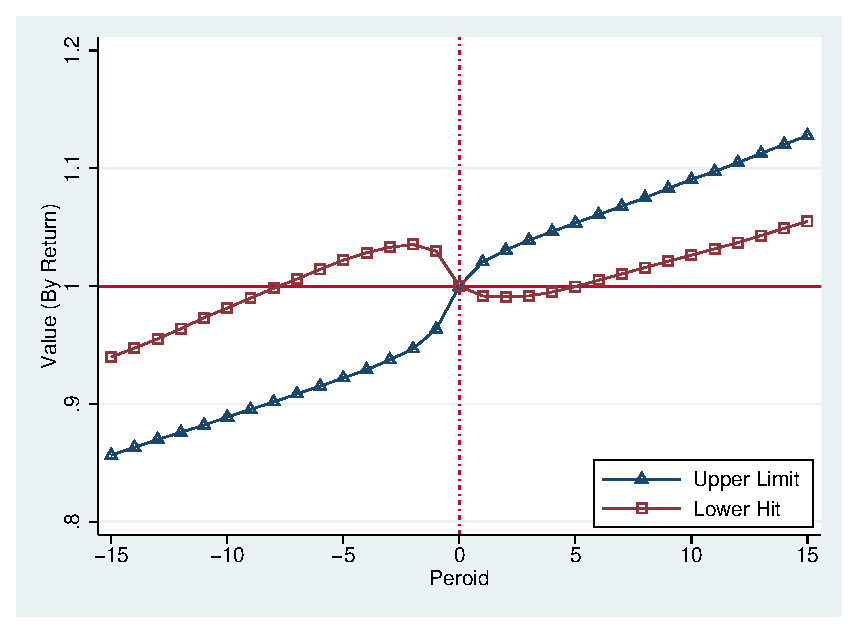
\includegraphics[width=0.8\columnwidth]{R.eps}
\caption{ارزش نماد از 15 دوره قبل  و بعد از برخورد  با توجه به بازده نماد }
\label{g4}
\end{figure}

\begin{figure}[htbp]
\centering
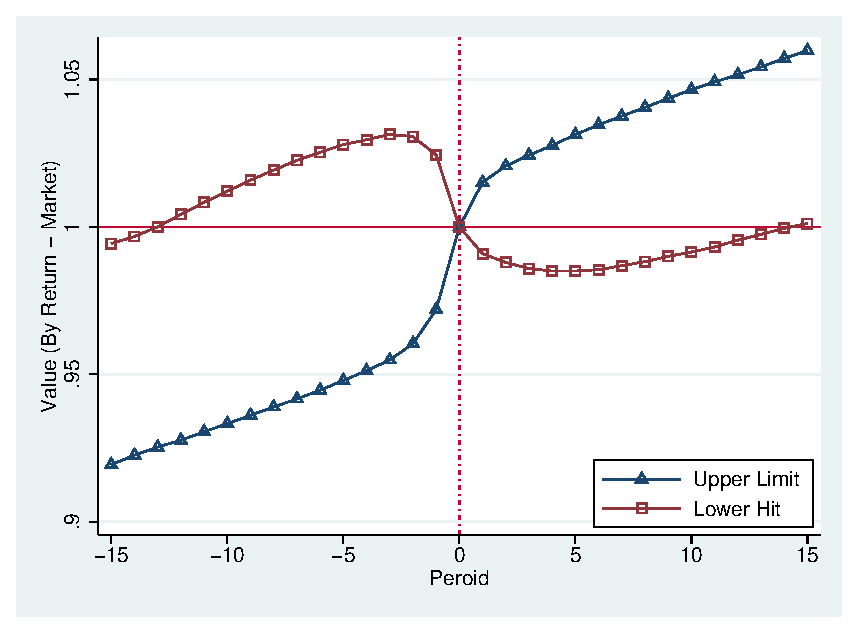
\includegraphics[width=0.8\columnwidth]{ER.eps}
\caption{ارزش نماد از 15 دوره قبل  و بعد از برخورد با توجه به بازده اضافی نماد }
\label{g5}
\end{figure}


یکی دیگر از تاثیرات برخورد قیمت به دامنه نوسان جلب نظر سرمایه‌گذاران حقیقی به نماد می‌باشد. با توجه به رابطه 
\ref{e1}
 ملاک عدم تعادل حقیقی و حقوقی 
در دو اتفاق برخورد به سقف و کف تعریف شده‌است.
 همانطور که در نمودار  
 \ref{g6}
 مشاهده می‌شود در حادثه برخورد قیمت به سقف نوسان خرید حقیقی در نماد افزایش پیدا می‌کند و از طرفی مالکان حقوقی در حال خروج از نماد می‌باشند. پس از برخورد به دامنه نوسان بعد از یک دوره این نسبت تغییر می‌کند و افراد حقیقی در حال خروج از نماد می‌باشند و حقوقی در حال خرید می‌باشد. با توجه به تعریف دو ملاک صورت دو ملاک قرینه یک‌دیگر می‌باشند. در نتیجه با توجه به اندازه نسبتا کم ملاک حقیقی می‌توان نتیجه گرفت عمده معاملات در این روز توسط افراد حقیقی انجام شده‌است. 
 
 در برخود قیمت به کف دامنه نوسان این رابطه عکس می‌باشد. در نمودار
 \ref{g7}
 رفتار عدم تعادل حقوقی و حقیقی برای نماد در زمان برخورد به کف قیمت رسم شده‌است. به صورت متوسط در روز برخورد قیمت به کف دامنه خریداران حقیقی افزایش قابل توجهی می‌یابند. اما برخلاف برخورد قیمت به سقف نوسان، بعد از برخورد به کف این رفتار حقیقی و حقوقی تغییر نمی‌کند و همچنان حقوقی فروشنده سهم می‌باشد و حقیقی در حال خرید می‌باشد. با توجه به توضیحات بند قبل با توجه به تعریف ملاک می‌توان نتیجه گرفت که در این روز وزن معاملات حقوقی نسبت به حقیقی بیشتر است.
 
\begin{figure}[htbp]
\centering
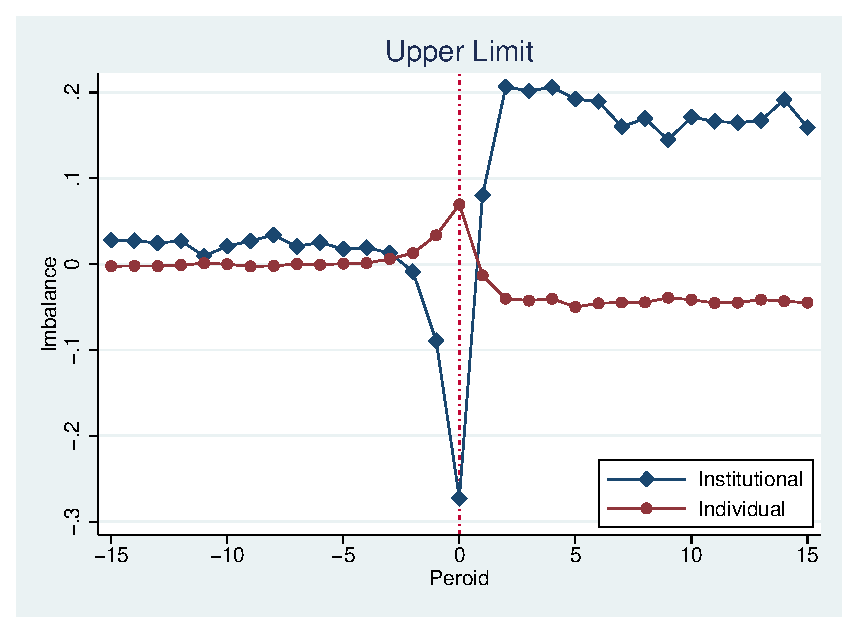
\includegraphics[width=0.8\columnwidth]{UI.eps}
\caption{عدم تعادل خرید و فروش حقیقی و حقوقی از 15 دوره قبل  و بعد از برخورد  به سقف دامنه }
\label{g6}
\end{figure}
\begin{figure}[htbp]
\centering
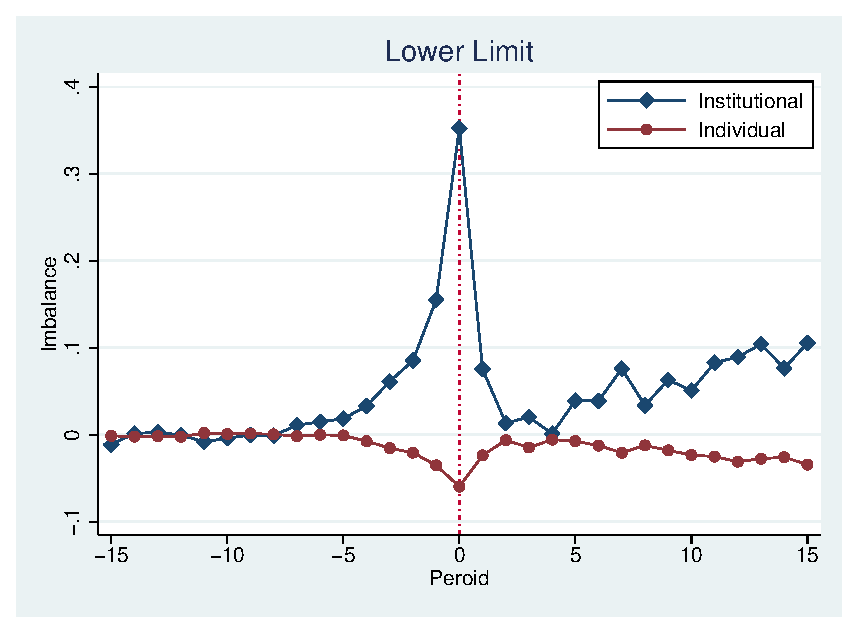
\includegraphics[width=0.8\columnwidth]{LI.eps}
\caption{عدم تعادل خرید و فروش حقیقی و حقوقی از 15 دوره قبل   و بعد از برخورد به کف دامنه }
\label{g7}
\end{figure}

یکی دیگر از تبعات مطرح‌شده در هنگام برخورد به دامنه نوسان، افزایش حجم معاملات در نماد می‌باشد. با توجه به دو تعریف مطرح شده در مقاله بخش
\ref{s1.1}
از ملاک 
Turn
و
RelTrun
با استفاده از رابطه 
\ref{e2}
و
\ref{e3}
دو ملاک فوق تعریف شده‌است. همانطور که در نمودار 
\ref{g8}
و
\ref{g8}
مشاهده می‌شود برخورد به قیمت به سقف دامنه نوسان تغییر چشم گیری در حجم معاملات اتفاق می‌افتد ولی این امر در کف دامنه نوسان صادق نمی‌باشد. دلیل امر به نظر می‌رسد برخورد به کف پایین دامنه نوسان اتفاق جذابی جهت جذب سرمایه گذاران به نماد نمی‌باشد و در عمل سبب افزایش حجم معاملات نمی‌باشد.   



\begin{figure}[htbp]
\centering
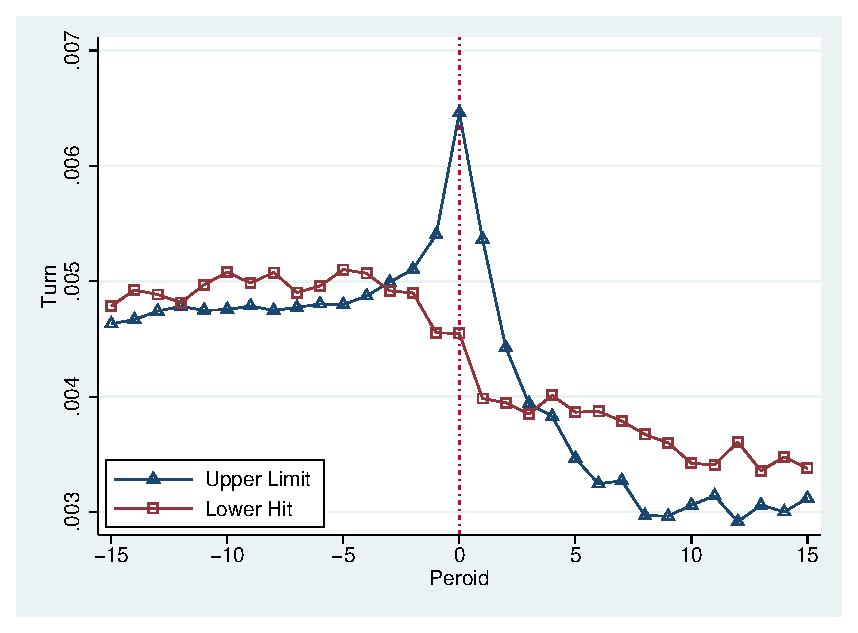
\includegraphics[width=0.8\columnwidth]{T.eps}
\caption{Turnover نماد 15 روز قبل و بعد از برخورد به دامنه نوسان}
\label{g8}
\end{figure}

\begin{figure}[htbp]
\centering
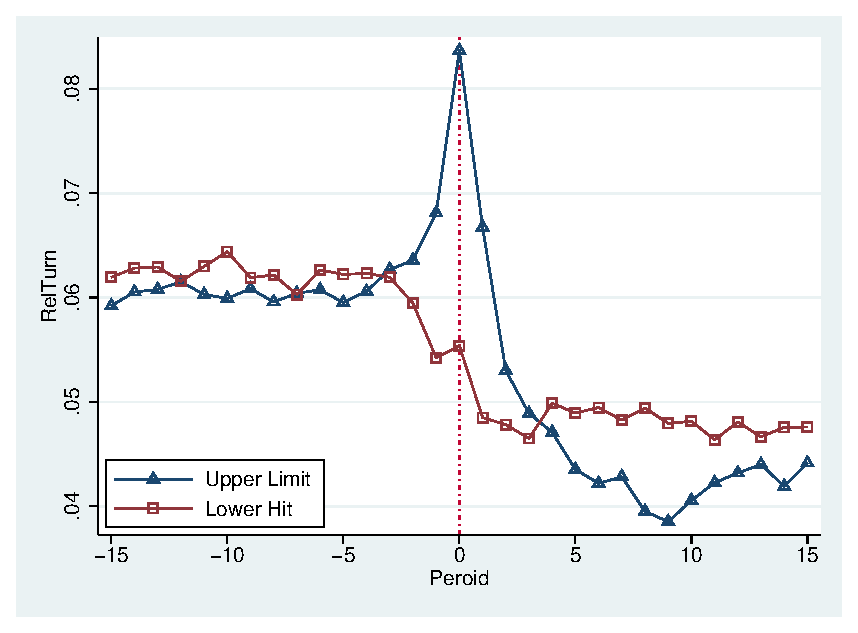
\includegraphics[width=0.8\columnwidth]{RT.eps}
\caption{\lr{Relative Turnover} نماد 15 روز قبل و بعد از برخورد به دامنه نوسان}
\label{g9}
\end{figure}
\FloatBarrier


\section{یافته‌های پژوهش}
با توجه به مقدمه مطرح شده وجود دامنه نوسان بر سه عامل مرتبط با نماد تاثیر می‌گذارد که در ادامه در هر بخش به هر یک از این مسائل پرداخته می‌شود.

\subsection{بازده}
در این بخش از متغیر‌های وابسته تعریف شده در جدول 
\ref{t1}
استفاده شده‌است و پس از آن به روش برآورد اثر ثابت در سطح نماد ضرایب مد نظر برآورد شده‌است. در جدول 
\ref{t3}
و
\ref{t11}
نتایج برآورد ضرایب به صورت مختصر آورده شده‌است که به ترتیب نحوه رفتار معامله‌گران و بازده نماد را مورد بررسی قرار می‌دهند.

در جدول شماره
\ref{t3}
ردیف شماره یک ضریب مدل به ازای برخود حداکثر قیمت به سقف دامنه نوسان را نشان می‌دهد. در اولین روز بازده روزانه نماد از اولین معامله تا قیمت پایانی نماد در آن روز برابر 
$ 0.8\% $
می‌باشد. بازده روزانه آخرین قیمت نسبت به اولین معامله نسبت به این عدد حدود یک و نیم درصد بیشتر ( بازده آخرین معامله نسبت به اولین معامله برابر است با 
$ 2\% $
) می‌باشد. به نظر می‌آید با توجه به نحوه محاسبه قیمت پایانی در این بازار و تشکیل صف در سقف، حجم مناسبی در این قیمت معامله نمی‌شود و سهامداران هنگام تشکیل صف تمایلی به فروش سهام خود ندارند. مقایسه این بازده برای هنگامی که قیمت به سقف برخورد نمی‌کند ولی به سقف نزدیک می‌شود  این نتیجه را تایید می‌کند.

در روز بعد اولین معامله نسبت به قیمت پایانی روز قبل با جهشی برابر 
$ 3.8\% $
مواجه می‌باشد که این مقدار حدود 
$ 2.6\% $
از آخرین معامله روز قبل بالا‌تر است. اما این رشد غیرمتعارف قیمت آغازین در ادامه این روز کاهش پیدا می‌کند و قیمت پایانی روز از این قیمت به مقدار 
$ 1.3\% $
کمتر است. اما آخرین قیمت معاملاتی این روز نسبت به قیمت پایانی آن به قیمت آغازین نزدیک‌تر است.
این مشاهدات با داده‌های موجود نیز سازگار می‌باشد. در شکل 
\ref{g10}
قیمت پایانی در روز قبل از برخورد به سقف دامنه یک فرض شده‌است و قیمت‌های پایانی و آغازین معاملات نسبت به این قیمت رسم شده‌است.
روند‌های فوق در این شکل نیز دیده می‌شوند.


 \begin{figure}[htbp]
 \centering
 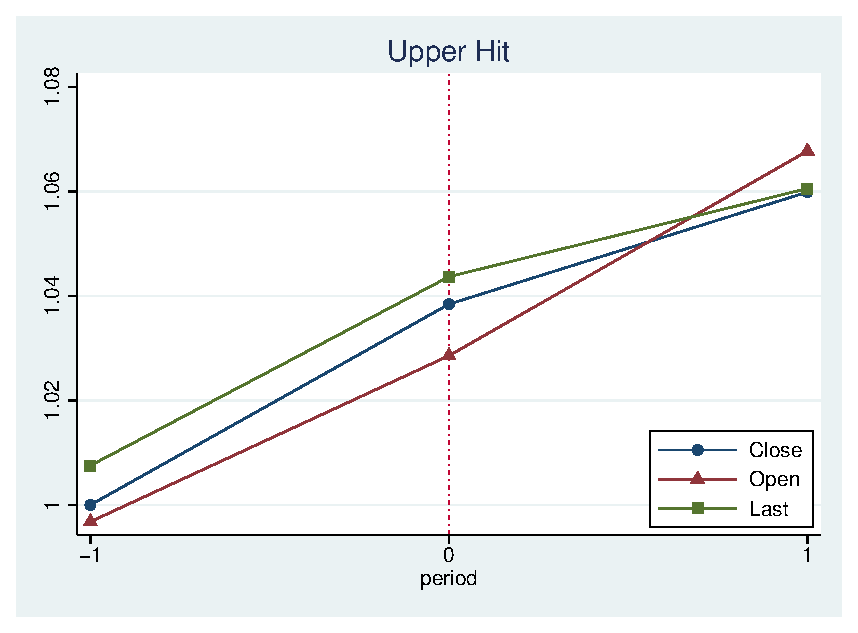
\includegraphics[width=0.8\columnwidth]{DUT.eps}
 \caption{ قیمت اولین  و آخرین معامله و قیمت پایانی در دوره 
  $ -1 $،
  0 
  و 
  1 
  برای برخورد به سقف دامنه}
 \label{g10}
 \end{figure}
 
 آخرین ردیف در جدول 
 \ref{t3}
 نیز ضریب مدل به ازای برخورد به کف دامنه نوسان می‌باشد. 
 در روز برخورد، بازده نماد از اولین معامله تا قیمت پایانی نماد در آن روز برابر
  $ -1.5\% $
  می‌باشد.
  بازده روزانه آخرین قیمت نسبت به اولین معامله نیز برابر 
   $ -1.8\% $
   می‌باشد که حدودا اختلافی
   $ 0.3\% $
   با بازده قبلی دارد. به نظر می‌آید برخلاف برخورد قیمت با سقف دامنه، در این اتفاق سهامداران تمایل به فروش سهام پیدا می‌کنند و به این دلیل قیمت پایانی به قیمت آخرین معامله نزدیک‌تر می‌شود.
 
 در روز بعد، اولین معامله نسبت به قیمت پایانی روز قبل با کاهش 
 $ 1\% $
 مواجه می‌باشد که این مقدار حدود 
 $ 0.4\% $
 از آخرین معامله روز قبل بیشتر کاهش پیدا کرده‌است. 
 اما این کاهش قیمت آغازین در ادامه این روز کاهش پیدا می‌کند و قیمت پایانی روز از این قیمت به مقدار 
 $0.5\% $
 بالا‌تر است. اما آخرین قیمت معاملاتی این روز نسبت به قیمت پایانی آن به قیمت آغازین نزدیک‌تر است.
 این مشاهدات با داده‌های موجود نیز سازگار می‌باشد. در شکل 
 \ref{g11}
 قیمت پایانی در روز قبل از برخورد به کف دامنه یک فرض شده‌است و قیمت‌های پایانی و آغازین معاملات نسبت به این قیمت رسم شده‌است.
 روند‌های فوق در این شکل نیز دیده می‌شوند.
 
 
  \begin{figure}[htbp]
  \centering
  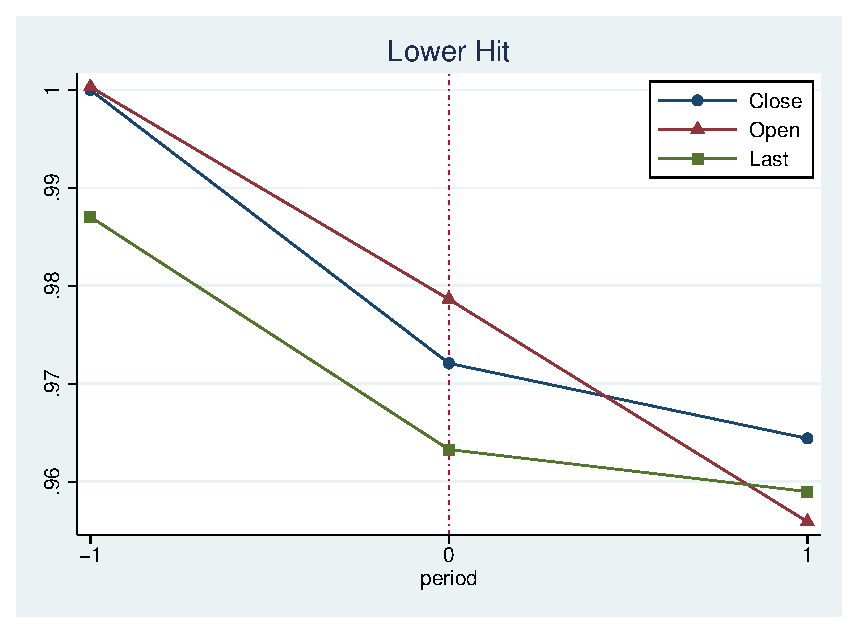
\includegraphics[width=0.8\columnwidth]{DLT.eps}
 \caption{ قیمت اولین  و آخرین معامله و قیمت پایانی در دوره 
 $ -1 $،
 0 
 و 
 1 
 برای برخورد به کف دامنه}
  \label{g11}
  \end{figure}
  
  در جدول 
  \ref{t11}
 رفتار بازده سهام مورد بررسی قرار گرفته‌است. در این جدول  
   ستون‌های 3 الی 6   بازده تجمیعی میان روز‌های نوشته شده را نمایندگی می‌کند. در این پژوهش از بازده های 2 الی 5، 5 الی 50 ، 50 الی 100 و 100 الی 300 روزه استفاده شده‌است. با توجه به نتایج جدول شماره 
   \ref{t3}
   همانطور که انتظار می‌رود برخورد به دامنه نوسان سبب تغییر رفتار بازده نماد می‌گردد. در ستون شماره یک به ازای برخورد به سقف دامنه نوسان بازده نماد حدود 3 برابر نسبت به عدم برخود افزایش پیدا می‌کند. در هنگام برخود به کف نیز همین نسبت برقرار است و صرفا در این حالت بازده سهام تقریبا با این نسبت کاهش پیدا می‌کند. این بازده چشم‌گیر تقریبا ادامه پیدا می‌کند و در ستون شماره شش که بازده تجمیعی 100 الی 300 روزه مورد بررسی قرار می‌گیرد برخورد به دامنه نوسان حدود سه برابر بازده بالا‌تر نسبت به عدم برخورد تولید می‌کند. در این بازده نماد برخورد کرده به کف دامنه نوسان بر می‌گردد و از برخود نکردن به سقف دامنه نوسان بازده‌ای به مراتب بیشتر از نماد برخورد کننده به سقف دامنه پیدا می‌کند. حدودا شش برابر از حالت برخورد نکردن به کف دامنه بازده بیشتری تولید می‌کند و حتی در این بازده از سهم برخورد کننده به سقف دامنه نیز بازده بالاتری دارد.
  
\newgeometry{top=10mm, bottom=20mm,left = 5mm,right = 5mm}
%\begin{landscape}

\begin{table}[htbp]
\centering
\begin{LTR}
\lr{{
\def\sym#1{\ifmmode^{#1}\else\(^{#1}\)\fi}
\begin{tabular}{l*{6}{c}}
\hline\hline
                    &\multicolumn{1}{c}{(1)}&\multicolumn{1}{c}{(2)}&\multicolumn{1}{c}{(3)}&\multicolumn{1}{c}{(4)}&\multicolumn{1}{c}{(5)}&\multicolumn{1}{c}{(6)}\\
                    &\multicolumn{1}{c}{Close-Open}&\multicolumn{1}{c}{Last-Open}&\multicolumn{1}{c}{TOpen-Last}&\multicolumn{1}{c}{TOpen-Close}&\multicolumn{1}{c}{TOpen-TClose}&\multicolumn{1}{c}{TLast-TOpen}\\
\hline
upperHit            &       0.792\sym{***}&       2.008\sym{***}&       2.587\sym{***}&       3.794\sym{***}&      -1.324\sym{***}&      -0.827\sym{***}\\
                    &      (7.82)         &     (50.88)         &     (68.59)         &     (55.65)         &    (-20.66)         &    (-32.13)         \\
[1em]
[4.5,5)             &       1.070\sym{***}&       1.408\sym{***}&       1.311\sym{***}&       1.662\sym{***}&      -0.270\sym{***}&      -0.222\sym{***}\\
                    &     (26.35)         &     (35.24)         &     (39.27)         &     (43.12)         &     (-8.14)         &     (-6.55)         \\
[1em]
[4,4.5)             &       0.227\sym{***}&       0.293\sym{***}&       0.138\sym{***}&       0.197\sym{***}&      -0.256\sym{***}&      -0.297\sym{***}\\
                    &      (6.57)         &      (7.24)         &      (4.72)         &      (6.31)         &     (-9.08)         &     (-9.25)         \\
[1em]
[2,4)               &      -0.934\sym{***}&      -0.247\sym{***}&       0.503\sym{***}&       1.167\sym{***}&      -0.701\sym{***}&      -0.221\sym{***}\\
                    &    (-14.08)         &     (-9.25)         &     (20.19)         &     (27.68)         &    (-17.79)         &    (-11.50)         \\
[1em]
(-2,2)              &      -0.985\sym{***}&      -0.375\sym{***}&       0.541\sym{***}&       1.133\sym{***}&      -0.505\sym{***}&     -0.0311         \\
                    &    (-15.40)         &    (-15.31)         &     (18.74)         &     (25.99)         &    (-12.70)         &     (-1.33)         \\
[1em]
(-4,-2]             &      -0.786\sym{***}&      -0.730\sym{***}&       0.395\sym{***}&       0.438\sym{***}&      -0.219\sym{***}&     -0.0744\sym{***}\\
                    &    (-23.69)         &    (-34.67)         &     (19.35)         &     (16.22)         &     (-9.22)         &     (-3.80)         \\
[1em]
(-4.5,-4]           &      -0.207\sym{***}&      -0.302\sym{***}&      0.0664\sym{*}  &     -0.0331         &      0.0519         &      0.0645\sym{*}  \\
                    &     (-6.49)         &     (-8.71)         &      (2.35)         &     (-1.04)         &      (1.90)         &      (2.13)         \\
[1em]
(-5,-4.5]           &      -0.505\sym{***}&      -0.530\sym{***}&      -0.192\sym{***}&      -0.198\sym{***}&       0.291\sym{***}&       0.241\sym{***}\\
                    &    (-12.18)         &    (-15.32)         &     (-5.98)         &     (-5.05)         &      (8.90)         &      (7.63)         \\
[1em]
lowerHit            &      -1.452\sym{***}&      -1.813\sym{***}&      -0.631\sym{***}&      -0.987\sym{***}&       0.464\sym{***}&       0.337\sym{***}\\
                    &    (-28.53)         &    (-47.08)         &    (-19.17)         &    (-27.25)         &     (13.36)         &     (10.44)         \\
[1em]
Constant            &       0.734\sym{***}&       0.107\sym{***}&      -0.402\sym{***}&      -1.012\sym{***}&       0.581\sym{***}&       0.157\sym{***}\\
                    &     (12.22)         &      (3.89)         &    (-13.26)         &    (-21.91)         &     (14.34)         &      (6.00)         \\
\hline
Observations        &      245107         &      245107         &      245105         &      245105         &      245103         &      245103         \\
\(R^{2}\)           &       0.083         &       0.138         &       0.102         &       0.176         &       0.048         &       0.016         \\
\hline\hline
\multicolumn{7}{l}{\footnotesize \textit{t} statistics in parentheses}\\
\multicolumn{7}{l}{\footnotesize \sym{*} \(p<0.05\), \sym{**} \(p<0.01\), \sym{***} \(p<0.001\)}\\
\end{tabular}
}
}
\end{LTR}
\caption{ضرایب برآورد رفتار معامله‌گران با در نظر گرفتن اثر ثابت در سطح نماد}
\label{t3}
\end{table}

%\end{landscape}
\begin{table}[htbp]
\centering
\begin{LTR}
\lr{{
\def\sym#1{\ifmmode^{#1}\else\(^{#1}\)\fi}
\begin{tabular}{l*{6}{c}}
\hline\hline
                    &\multicolumn{1}{c}{(1)}&\multicolumn{1}{c}{(2)}&\multicolumn{1}{c}{(3)}&\multicolumn{1}{c}{(4)}&\multicolumn{1}{c}{(5)}&\multicolumn{1}{c}{(6)}\\
                    &\multicolumn{1}{c}{Ret\_1}&\multicolumn{1}{c}{Ret\_2}&\multicolumn{1}{c}{[2,5]}&\multicolumn{1}{c}{[5,50]}&\multicolumn{1}{c}{[50,100]}&\multicolumn{1}{c}{[100,300]}\\
\hline
upperHit            &       1.856\sym{***}&       2.732\sym{***}&       1.714\sym{***}&       20.44\sym{***}&       8.055\sym{***}&       117.4\sym{***}\\
                    &     (60.81)         &     (41.73)         &     (17.21)         &     (17.28)         &      (3.38)         &      (7.71)         \\
[1em]
[4.5,5)             &       1.269\sym{***}&       1.703\sym{***}&       0.696\sym{***}&       0.223         &       1.873         &      -10.31         \\
                    &     (38.33)         &     (30.29)         &      (8.50)         &      (0.32)         &      (1.54)         &     (-1.51)         \\
[1em]
[4,4.5)             &     -0.0932\sym{**} &      -0.196\sym{***}&     -0.0282         &       2.060\sym{***}&       3.051\sym{**} &       30.31\sym{***}\\
                    &     (-3.13)         &     (-3.97)         &     (-0.39)         &      (3.88)         &      (3.24)         &      (5.07)         \\
[1em]
[2,4)               &     -0.0102         &       0.141\sym{***}&       0.532\sym{***}&       5.174\sym{***}&       8.859\sym{***}&       43.64\sym{***}\\
                    &     (-0.51)         &      (3.78)         &      (9.43)         &     (13.34)         &     (12.44)         &      (9.37)         \\
[1em]
(-2,2)              &      -0.230\sym{***}&      -0.170\sym{***}&     -0.0426         &      -2.881\sym{***}&       1.380         &      -13.45\sym{**} \\
                    &     (-9.33)         &     (-3.44)         &     (-0.57)         &     (-5.10)         &      (1.43)         &     (-2.63)         \\
[1em]
(-4,-2]             &      -0.491\sym{***}&      -0.562\sym{***}&      -0.122\sym{*}  &       2.454\sym{***}&       6.004\sym{***}&       21.34\sym{***}\\
                    &    (-22.94)         &    (-13.72)         &     (-2.07)         &      (6.27)         &      (8.93)         &      (4.90)         \\
[1em]
(-4.5,-4]           &     -0.0236         &     0.00775         &     -0.0253         &       2.317\sym{***}&       1.121         &       15.28\sym{**} \\
                    &     (-0.78)         &      (0.16)         &     (-0.37)         &      (4.50)         &      (1.42)         &      (3.08)         \\
[1em]
(-5,-4.5]           &      -0.564\sym{***}&      -0.908\sym{***}&      -0.669\sym{***}&      -0.485         &       2.315\sym{*}  &      -7.919         \\
                    &    (-18.13)         &    (-17.76)         &     (-9.23)         &     (-0.76)         &      (2.37)         &     (-1.49)         \\
[1em]
lowerHit            &      -1.333\sym{***}&      -1.781\sym{***}&      -0.609\sym{***}&       8.191\sym{***}&       13.20\sym{***}&       28.82\sym{**} \\
                    &    (-42.83)         &    (-28.01)         &     (-6.26)         &      (7.56)         &      (6.16)         &      (3.17)         \\
[1em]
Up Market           &      0.0615\sym{***}&    -0.00688         &       0.129\sym{***}&       0.831\sym{***}&       3.174\sym{***}&      -9.868\sym{***}\\
                    &      (5.09)         &     (-0.33)         &      (4.57)         &      (3.56)         &      (8.07)         &     (-4.80)         \\
[1em]
Constant            &       0.394\sym{***}&       0.892\sym{***}&       1.445\sym{***}&       26.24\sym{***}&       41.06\sym{***}&       313.2\sym{***}\\
                    &     (14.82)         &     (15.47)         &     (15.28)         &     (16.55)         &     (15.74)         &     (20.68)         \\
\hline
Observations        &      304849         &      304400         &      303053         &      282856         &      260512         &      174360         \\
\(R^{2}\)           &       0.082         &       0.060         &       0.014         &       0.032         &       0.017         &       0.019         \\
\hline\hline
\multicolumn{7}{l}{\footnotesize \textit{t} statistics in parentheses}\\
\multicolumn{7}{l}{\footnotesize This table reports fixed effect estimates of normal returns.}\\
\multicolumn{7}{l}{\footnotesize The independent variables are dummies that control for events . We calculate standard errors by using fixed effect on stock level}\\
\multicolumn{7}{l}{\footnotesize \sym{*} \(p<0.05\), \sym{**} \(p<0.01\), \sym{***} \(p<0.001\)}\\
\end{tabular}
}
}
\end{LTR}
\caption{ضرایب برآورد بازده خالص با در نظر گرفتن اثر ثابت در سطح نماد}
\label{t11}
\end{table}

\restoregeometry






\subsection{حجم}

در این بخش با استفاده متغیر‌های وابسته تعریف شده در بخش 
\ref{s1.1}
اثر برخورد به دامنه نوسان بررسی می‌شود. به این منظور روابط 
\ref{e2} 
و
\ref{e3}
به صورت زیر بازنویسی می‌شوند.

\lr{\begin{align*}
\text{Turn}_{k,t} = \frac{\text{Volume}(\text{Rial})_{k,t}}{\text{MarketCap(FreeFloat)}_{k,t}}\\\\
\text{RelTurn}_{k,t} = \frac{\text{Turn}_{k,t}}{AVG(\text{Turn}_{k,t})}
\end{align*}}
 علاوه بر روابط فوق از لگاریتم طبیعی حجم معاملات، نیز به عنوان متغیر وابسته استفاده شده‌است. به این منظور ضرایب با کنترل اثر ثابت در سطح هر نماد، برآورد شده‌اند و نتایج برآورد در جدول 
 \ref{t5}
 بیان شده‌است. با توجه به این جدول  روند افزایش حجم هر آنچه از 
$  2 \% $
 به بالا حرکت می‌کنیم افزایش پیدا می‌کند و با 
 برخورد قیمت به سقف دامنه، به صورت متوسط حجم معاملات
  $ 150\% $
  افزایش پیدا می‌کند. 
 با برخورد قیمت به کف دامنه نیز حجم معاملات به طور متوسط 
  $ 81\% $
  افزایش پیدا می‌کند. همانطور که از شکل 
  \ref{g8}
  و
  \ref{g9}
  انتظار داشتیم نزدیک شدن به کف دامنه تاثیری به اندازه برخود به سقف دامنه بر حجم معاملات نمی‌گذارد.
  با دیگر ملاک‌های بررسی حجم معاملات نیز می‌توان اثرات فوق را در حجم معاملات پیدا کرد.
 


\newgeometry{top=10mm, bottom=15mm,left = 5mm,right = 5mm}
%\begin{landscape}

\begin{table}[htbp]
\centering
\begin{LTR}
\lr{{
\def\sym#1{\ifmmode^{#1}\else\(^{#1}\)\fi}
\begin{tabular}{l*{3}{c}}
\hline\hline
                    &\multicolumn{1}{c}{(1)}&\multicolumn{1}{c}{(2)}&\multicolumn{1}{c}{(3)}\\
                    &\multicolumn{1}{c}{lnvolume}&\multicolumn{1}{c}{Turn}&\multicolumn{1}{c}{RelTurn}\\
\hline
upperHit            &       2.179\sym{***}&     0.00636\sym{***}&       1.107\sym{***}\\
                    &     (44.82)         &     (20.34)         &     (49.38)         \\
[1em]
[4.5,5)             &       0.724\sym{***}&     0.00286\sym{***}&       0.599\sym{***}\\
                    &     (37.13)         &     (14.50)         &     (35.42)         \\
[1em]
[4,4.5)             &       0.402\sym{***}&    0.000999\sym{***}&       0.161\sym{***}\\
                    &     (24.09)         &      (8.14)         &     (12.51)         \\
[1em]
[2,4)               &       0.878\sym{***}&     0.00215\sym{***}&       0.288\sym{***}\\
                    &     (31.82)         &     (16.60)         &     (24.34)         \\
[1em]
(-2,2)              &     -0.0289         &     0.00210\sym{***}&      0.0713\sym{***}\\
                    &     (-1.05)         &     (11.53)         &      (4.03)         \\
[1em]
(-4,-2]             &       0.519\sym{***}&     0.00205\sym{***}&       0.144\sym{***}\\
                    &     (28.90)         &     (16.42)         &     (10.31)         \\
[1em]
(-4.5,-4]           &       0.305\sym{***}&     0.00111\sym{***}&      0.0821\sym{***}\\
                    &     (16.63)         &      (4.00)         &      (6.54)         \\
[1em]
(-5,-4.5]           &       0.376\sym{***}&     0.00124\sym{***}&       0.145\sym{***}\\
                    &     (13.39)         &      (4.88)         &     (11.01)         \\
[1em]
lowerHit            &       1.429\sym{***}&     0.00480\sym{***}&       0.514\sym{***}\\
                    &     (37.04)         &     (17.73)         &     (26.49)         \\
[1em]
Up Market           &       0.268\sym{***}&    0.000737\sym{***}&       0.122\sym{***}\\
                    &     (26.43)         &      (6.88)         &     (18.54)         \\
[1em]
Constant            &       12.32\sym{***}&    -0.00120\sym{***}&       0.394\sym{***}\\
                    &    (280.83)         &     (-4.05)         &     (19.25)         \\
\hline
Observations        &      305297         &      305298         &      305298         \\
\(R^{2}\)           &       0.225         &       0.028         &       0.068         \\
\hline\hline
\multicolumn{4}{l}{\footnotesize \textit{t} statistics in parentheses}\\
\multicolumn{4}{l}{\footnotesize This table reports fixed effect estimates of volume, turnover and relative turnover.}\\
\multicolumn{4}{l}{\footnotesize The independent variables are dummies that control for events . We calculate standard errors by using fixed effect on stock level}\\
\multicolumn{4}{l}{\footnotesize \sym{*} \(p<0.05\), \sym{**} \(p<0.01\), \sym{***} \(p<0.001\)}\\
\end{tabular}
}
}
\end{LTR}
\caption{ضرایب برآورد متغیر‌های کنترل‌کننده حجم با در نظر گرفتن اثر ثابت در سطح نماد}
\label{t5}
\end{table}


%\end{landscape}
\restoregeometry
\FloatBarrier

\subsection{خرید حقیقی و حقوقی}
در این بخش با استفاده از رابطه‌ی تعریف شده جهت بررسی تغییرات خرید و فروش سهامداران حقیقی و حقوقی به بررسی رفتار سهام‌داران حقیقی و حقوی می‌پردازیم.
با توجه  
\ref{e1} 
برای سرمایه‌گذاران حقیقی و حقوقی داریم:
\begin{align*}
\text{Imbalance}_{k,t}^{\text{Indiv}} = \frac{\text{Buys}_{k,t}^{\text{Indiv}} - \text{Sells}_{k,t}^{\text{Indiv}}}{\text{Buys}_{k,t}^{\text{Indiv}} + \text{Sells}_{k,t}^{\text{Indiv}}}\\\\
\text{Imbalance}_{k,t}^{\text{Inst}} = \frac{\text{Buys}_{k,t}^{\text{Inst}} - \text{Sells}_{k,t}^{\text{Inst}}}{\text{Buys}_{k,t}^{\text{Inst}} + \text{Sells}_{k,t}^{\text{Inst}}}
\end{align*}
که در ادامه به ترتیب به صورت 
$ \text{IndlImbalance}  $
و
$ \text{InslImbalance} $
استفاده می‌شوند.
بر همین اساس برای دوره $ t+1 $ نیز این شاخص‌ها تعریف شده‌است که به ترتیب به صورت 
$ \text{FIndlImbalance}  $
و
$ \text{FInslImbalance} $
نشان داده می‌شود.

نتایج برآورد ضرایب با در نظر گرفتن اثر ثابت در سطح نماد، در جدول 
\ref{t6}
آورده شده‌است. همانطور که از شکل 
\ref{g6}
انتظار داشتیم با برخود به سقف دامنه، سهامداران حقوقی سهم کاهش پیدا می‌کند و سهام‌داران حقیقی نماد افزایش پیدا می‌کنند. 
این افزایش در سهامداران حقیقی و کاهش در سهام داران حقوقی تا فردا نیز ادامه پیدا می‌کند. 

\newgeometry{top=10mm, bottom=15mm,left = 5mm,right = 5mm}
%\begin{landscape}

\begin{table}[htbp]
\centering
\begin{LTR}
\lr{{
\def\sym#1{\ifmmode^{#1}\else\(^{#1}\)\fi}
\begin{tabular}{l*{4}{c}}
\hline\hline
                    &\multicolumn{1}{c}{(1)}&\multicolumn{1}{c}{(2)}&\multicolumn{1}{c}{(3)}&\multicolumn{1}{c}{(4)}\\
                    &\multicolumn{1}{c}{InslImbalance}&\multicolumn{1}{c}{FInslImbalance}&\multicolumn{1}{c}{IndlImbalance}&\multicolumn{1}{c}{FIndlImbalance}\\
\hline
upperHit            &      -0.603\sym{***}&      -0.325\sym{***}&       0.141\sym{***}&      0.0910\sym{***}\\
                    &    (-38.54)         &    (-24.89)         &     (21.03)         &     (16.91)         \\
[1em]
[4.5,5)             &      -0.256\sym{***}&      -0.160\sym{***}&      0.0697\sym{***}&      0.0403\sym{***}\\
                    &    (-22.62)         &    (-13.71)         &     (19.08)         &     (13.32)         \\
[1em]
[4,4.5)             &     -0.0778\sym{***}&     -0.0128         &      0.0117\sym{***}&     0.00778\sym{**} \\
                    &     (-7.76)         &     (-1.21)         &      (4.85)         &      (2.98)         \\
[1em]
[2,4)               &      -0.169\sym{***}&     -0.0770\sym{***}&      0.0280\sym{***}&      0.0216\sym{***}\\
                    &    (-23.23)         &    (-10.62)         &     (10.07)         &      (9.09)         \\
[1em]
(-2,2)              &     -0.0540\sym{***}&     -0.0383\sym{***}&     -0.0189\sym{***}&     -0.0110\sym{*}  \\
                    &     (-5.06)         &     (-3.81)         &     (-3.51)         &     (-2.24)         \\
[1em]
(-4,-2]             &    -0.00104         &     -0.0260\sym{***}&   -0.000676         &     0.00323         \\
                    &     (-0.17)         &     (-4.40)         &     (-0.30)         &      (1.66)         \\
[1em]
(-4.5,-4]           &      0.0120         &     -0.0157         &     0.00840\sym{***}&     0.00590\sym{*}  \\
                    &      (1.29)         &     (-1.52)         &      (3.66)         &      (2.19)         \\
[1em]
(-5,-4.5]           &     -0.0152         &     -0.0357\sym{***}&      0.0166\sym{***}&      0.0145\sym{***}\\
                    &     (-1.46)         &     (-3.38)         &      (6.08)         &      (4.98)         \\
[1em]
lowerHit            &       0.110\sym{***}&     -0.0239\sym{*}  &     0.00298         &      0.0173\sym{***}\\
                    &      (8.38)         &     (-2.00)         &      (0.64)         &      (3.99)         \\
[1em]
Constant            &       0.314\sym{***}&       0.227\sym{***}&     -0.0699\sym{***}&     -0.0564\sym{***}\\
                    &     (24.73)         &     (17.17)         &     (-9.91)         &     (-7.85)         \\
\hline
Observations        &      176979         &      176740         &      245076         &      244653         \\
\(R^{2}\)           &       0.083         &       0.021         &       0.046         &       0.020         \\
\hline\hline
\multicolumn{5}{l}{\footnotesize \textit{t} statistics in parentheses}\\
\multicolumn{5}{l}{\footnotesize \sym{*} \(p<0.05\), \sym{**} \(p<0.01\), \sym{***} \(p<0.001\)}\\
\end{tabular}
}
}
\end{LTR}
\caption{ضرایب برآورد عدم تعادل حقیقی و حقوقی با در نظر گرفتن اثر ثابت در سطح نماد}\label{t6}
\end{table}

%\end{landscape}
\restoregeometry



\begin{appendices}
\section{برآورد‌های محتلف سنجی}
\newgeometry{top=10mm, bottom=20mm,left = 5mm,right = 5mm}
\begin{LTR}
\begin{table}[htbp]
\centering
\lr{{
\def\sym#1{\ifmmode^{#1}\else\(^{#1}\)\fi}
\begin{tabular}{l*{6}{c}}
\hline\hline
                    &\multicolumn{1}{c}{(1)}&\multicolumn{1}{c}{(2)}&\multicolumn{1}{c}{(3)}&\multicolumn{1}{c}{(4)}&\multicolumn{1}{c}{(5)}&\multicolumn{1}{c}{(6)}\\
                    &\multicolumn{1}{c}{ERet\_1}&\multicolumn{1}{c}{ERet\_2}&\multicolumn{1}{c}{E[2,5]}&\multicolumn{1}{c}{E[5,50]}&\multicolumn{1}{c}{E[50,100]}&\multicolumn{1}{c}{E[100,300]}\\
\hline
upperHit            &       1.309\sym{***}&       1.711\sym{***}&       0.450\sym{**} &      -1.308         &      -5.469\sym{*}  &      -5.517         \\
                    &     (16.00)         &     (12.61)         &      (2.82)         &     (-0.76)         &     (-2.38)         &     (-0.80)         \\
[1em]
[4.5,5)             &       0.991\sym{***}&       1.230\sym{***}&       0.116         &      -4.449\sym{***}&      -6.643\sym{***}&      -0.442         \\
                    &     (22.09)         &     (16.77)         &      (1.21)         &     (-6.84)         &     (-5.44)         &     (-0.07)         \\
[1em]
[4,4.5)             &      -0.153\sym{***}&      -0.317\sym{***}&      -0.208\sym{**} &      -0.378         &      -0.406         &       11.43\sym{*}  \\
                    &     (-4.56)         &     (-5.67)         &     (-2.85)         &     (-0.77)         &     (-0.46)         &      (2.16)         \\
[1em]
[2,4)               &     -0.0498         &      0.0487         &       0.300\sym{***}&       1.737\sym{**} &       1.490         &       15.09\sym{***}\\
                    &     (-1.03)         &      (0.63)         &      (3.45)         &      (2.73)         &      (1.44)         &      (3.56)         \\
[1em]
(-2,2)              &      -0.202\sym{***}&      -0.212\sym{*}  &     -0.0745         &      -2.274\sym{*}  &      -2.981         &      -10.04\sym{*}  \\
                    &     (-3.61)         &     (-2.30)         &     (-0.68)         &     (-2.36)         &     (-1.77)         &     (-2.18)         \\
[1em]
(-4,-2]             &      -0.471\sym{***}&      -0.550\sym{***}&      -0.184\sym{*}  &      -0.329         &      -0.943         &       8.681\sym{*}  \\
                    &    (-10.21)         &     (-7.64)         &     (-2.23)         &     (-0.49)         &     (-0.89)         &      (2.05)         \\
[1em]
(-4.5,-4]           &      -0.112\sym{**} &      -0.146\sym{**} &      -0.192\sym{*}  &      -0.453         &      -0.160         &       7.599         \\
                    &     (-3.22)         &     (-2.68)         &     (-2.57)         &     (-0.90)         &     (-0.19)         &      (1.47)         \\
[1em]
(-5,-4.5]           &      -0.401\sym{***}&      -0.695\sym{***}&      -0.515\sym{***}&      -3.536\sym{***}&      -4.029\sym{**} &       7.654         \\
                    &     (-6.50)         &     (-6.98)         &     (-4.11)         &     (-4.33)         &     (-2.88)         &      (1.29)         \\
[1em]
lowerHit            &      -1.293\sym{***}&      -1.802\sym{***}&      -0.888\sym{***}&      -4.244\sym{*}  &      -3.797         &       19.36         \\
                    &    (-14.65)         &    (-12.74)         &     (-4.71)         &     (-2.19)         &     (-1.47)         &      (1.88)         \\
[1em]
Up Market           &      -0.548\sym{***}&      -0.733\sym{***}&      -0.287         &      -2.791\sym{*}  &      -3.977         &      -20.70\sym{*}  \\
                    &     (-8.08)         &     (-6.29)         &     (-1.86)         &     (-2.20)         &     (-1.63)         &     (-2.37)         \\
[1em]
Constant            &       0.449\sym{***}&       0.627\sym{***}&       0.468\sym{**} &      -0.400         &       2.922         &       14.21         \\
                    &      (5.35)         &      (4.55)         &      (2.79)         &     (-0.29)         &      (1.33)         &      (1.59)         \\
\hline
Observations        &      304849         &      304400         &      303053         &      282856         &      260512         &      174360         \\
\(R^{2}\)           &       0.048         &       0.033         &       0.004         &       0.004         &       0.003         &       0.029         \\
\hline\hline
\multicolumn{7}{l}{\footnotesize \textit{t} statistics in parentheses}\\
\multicolumn{7}{l}{\footnotesize This table reports OLS estimates of extra return from market.}\\
\multicolumn{7}{l}{\footnotesize The independent variables are dummies that control for events . We calculate standard errors by clustering on each stocks}\\
\multicolumn{7}{l}{\footnotesize \sym{*} \(p<0.05\), \sym{**} \(p<0.01\), \sym{***} \(p<0.001\)}\\
\end{tabular}
}
}
\caption{OLS regression of excess return, Clustered by calendar date}
\label{t4}
\end{table}

\end{LTR}
\restoregeometry


\newgeometry{top=10mm, bottom=20mm,left = 5mm,right = 5mm}
%\begin{landscape}
\begin{LTR}
\begin{table}[htbp]
\centering
\lr{{
\def\sym#1{\ifmmode^{#1}\else\(^{#1}\)\fi}
\begin{tabular}{l*{6}{c}}
\hline\hline
                    &\multicolumn{1}{c}{(1)}&\multicolumn{1}{c}{(2)}&\multicolumn{1}{c}{(3)}&\multicolumn{1}{c}{(4)}&\multicolumn{1}{c}{(5)}&\multicolumn{1}{c}{(6)}\\
                    &\multicolumn{1}{c}{ERet\_1}&\multicolumn{1}{c}{ERet\_2}&\multicolumn{1}{c}{E[2,5]}&\multicolumn{1}{c}{E[5,50]}&\multicolumn{1}{c}{E[50,100]}&\multicolumn{1}{c}{E[100,300]}\\
\hline
upperHit            &       1.306\sym{***}&       1.680\sym{***}&       0.357\sym{***}&      -3.365\sym{**} &      -7.211\sym{***}&      -47.00\sym{***}\\
                    &     (42.20)         &     (25.72)         &      (3.64)         &     (-2.82)         &     (-3.52)         &     (-3.39)         \\
[1em]
[4.5,5)             &       0.991\sym{***}&       1.220\sym{***}&      0.0828         &      -5.042\sym{***}&      -7.035\sym{***}&      -8.743         \\
                    &     (29.90)         &     (21.42)         &      (1.05)         &     (-8.09)         &     (-6.33)         &     (-1.50)         \\
[1em]
[4,4.5)             &      -0.153\sym{***}&      -0.317\sym{***}&      -0.209\sym{**} &      -0.437         &      -0.295         &       9.666         \\
                    &     (-5.34)         &     (-6.41)         &     (-2.97)         &     (-0.94)         &     (-0.34)         &      (1.87)         \\
[1em]
[2,4)               &     -0.0536\sym{**} &      0.0377         &       0.277\sym{***}&       1.157\sym{**} &       0.275         &      -1.784         \\
                    &     (-2.62)         &      (0.99)         &      (4.93)         &      (3.20)         &      (0.42)         &     (-0.46)         \\
[1em]
(-2,2)              &      -0.193\sym{***}&      -0.186\sym{***}&     -0.0201         &      -1.766\sym{***}&      -3.092\sym{***}&      -12.93\sym{**} \\
                    &     (-7.74)         &     (-3.83)         &     (-0.28)         &     (-3.39)         &     (-3.72)         &     (-3.01)         \\
[1em]
(-4,-2]             &      -0.476\sym{***}&      -0.559\sym{***}&      -0.192\sym{***}&      -0.444         &      -1.701\sym{**} &      -5.690         \\
                    &    (-22.14)         &    (-14.27)         &     (-3.39)         &     (-1.19)         &     (-2.67)         &     (-1.55)         \\
[1em]
(-4.5,-4]           &      -0.113\sym{***}&      -0.149\sym{**} &      -0.200\sym{**} &      -0.645         &      -0.407         &       2.539         \\
                    &     (-3.48)         &     (-3.12)         &     (-3.08)         &     (-1.40)         &     (-0.56)         &      (0.64)         \\
[1em]
(-5,-4.5]           &      -0.403\sym{***}&      -0.704\sym{***}&      -0.535\sym{***}&      -3.536\sym{***}&      -3.721\sym{***}&       4.567         \\
                    &    (-12.44)         &    (-14.04)         &     (-7.86)         &     (-6.21)         &     (-4.09)         &      (0.96)         \\
[1em]
lowerHit            &      -1.308\sym{***}&      -1.843\sym{***}&      -0.961\sym{***}&      -5.154\sym{***}&      -5.280\sym{**} &      -14.60\sym{*}  \\
                    &    (-40.29)         &    (-29.04)         &    (-10.65)         &     (-5.30)         &     (-2.74)         &     (-2.01)         \\
[1em]
Up Market           &      -0.549\sym{***}&      -0.734\sym{***}&      -0.285\sym{***}&      -2.642\sym{***}&      -3.661\sym{***}&      -19.54\sym{***}\\
                    &    (-40.29)         &    (-32.18)         &     (-9.23)         &    (-10.91)         &     (-9.33)         &    (-10.41)         \\
[1em]
Constant            &       0.503\sym{***}&       0.770\sym{***}&       0.764\sym{***}&       3.683\sym{**} &       7.500\sym{***}&       45.71\sym{***}\\
                    &     (17.56)         &     (13.28)         &      (8.27)         &      (2.90)         &      (3.63)         &      (3.61)         \\
\hline
Observations        &      304849         &      304400         &      303053         &      282856         &      260512         &      174360         \\
\(R^{2}\)           &       0.048         &       0.033         &       0.005         &       0.007         &       0.004         &       0.013         \\
\hline\hline
\multicolumn{7}{l}{\footnotesize \textit{t} statistics in parentheses}\\
\multicolumn{7}{l}{\footnotesize This table reports fixed effect estimates of extra return from market.}\\
\multicolumn{7}{l}{\footnotesize The independent variables are dummies that control for events . We calculate standard errors by using fixed effect on stock level}\\
\multicolumn{7}{l}{\footnotesize \sym{*} \(p<0.05\), \sym{**} \(p<0.01\), \sym{***} \(p<0.001\)}\\
\end{tabular}
}
}
\caption{FE of excess return, Fixed effect by firm}
\label{t8}
\end{table}
\end{LTR}
%\end{landscape}
\restoregeometry

\newgeometry{top=10mm, bottom=20mm,left = 5mm,right = 5mm}
%\begin{landscape}
\begin{LTR}
\begin{table}[htbp]
\centering
\lr{{
\def\sym#1{\ifmmode^{#1}\else\(^{#1}\)\fi}
\begin{tabular}{l*{6}{c}}
\hline\hline
                    &\multicolumn{1}{c}{(1)}&\multicolumn{1}{c}{(2)}&\multicolumn{1}{c}{(3)}&\multicolumn{1}{c}{(4)}&\multicolumn{1}{c}{(5)}&\multicolumn{1}{c}{(6)}\\
                    &\multicolumn{1}{c}{Close-Open}&\multicolumn{1}{c}{Last-Open}&\multicolumn{1}{c}{TOpen-Last}&\multicolumn{1}{c}{TOpen-Close}&\multicolumn{1}{c}{TOpen-TClose}&\multicolumn{1}{c}{TLast-TOpen}\\
\hline
upperHit            &       0.769\sym{***}&       2.003\sym{***}&       2.573\sym{***}&       3.799\sym{***}&      -1.333\sym{***}&      -0.807\sym{***}\\
                    &     (12.82)         &     (27.96)         &     (38.69)         &     (53.22)         &    (-24.23)         &    (-11.91)         \\
[1em]
[4.5,5)             &       1.083\sym{***}&       1.414\sym{***}&       1.308\sym{***}&       1.652\sym{***}&      -0.259\sym{***}&      -0.218\sym{***}\\
                    &     (28.46)         &     (30.21)         &     (30.63)         &     (32.83)         &     (-7.64)         &     (-5.10)         \\
[1em]
[4,4.5)             &       0.239\sym{***}&       0.297\sym{***}&       0.133\sym{***}&       0.185\sym{***}&      -0.246\sym{***}&      -0.293\sym{***}\\
                    &      (6.86)         &      (6.52)         &      (4.51)         &      (5.18)         &     (-7.54)         &     (-7.51)         \\
[1em]
[2,4)               &      -0.983\sym{***}&      -0.262\sym{***}&       0.504\sym{***}&       1.199\sym{***}&      -0.738\sym{***}&      -0.219\sym{***}\\
                    &    (-17.27)         &     (-4.01)         &     (12.96)         &     (25.25)         &    (-24.25)         &     (-6.37)         \\
[1em]
(-2,2)              &      -0.994\sym{***}&      -0.340\sym{***}&       0.512\sym{***}&       1.149\sym{***}&      -0.525\sym{***}&    -0.00735         \\
                    &    (-17.52)         &     (-5.37)         &      (7.38)         &     (16.63)         &    (-15.41)         &     (-0.19)         \\
[1em]
(-4,-2]             &      -0.768\sym{***}&      -0.715\sym{***}&       0.383\sym{***}&       0.423\sym{***}&      -0.207\sym{***}&     -0.0646\sym{*}  \\
                    &    (-19.74)         &    (-15.15)         &     (14.07)         &     (12.89)         &     (-9.60)         &     (-2.56)         \\
[1em]
(-4.5,-4]           &      -0.185\sym{***}&      -0.292\sym{***}&      0.0583\sym{*}  &     -0.0518         &      0.0671\sym{*}  &      0.0697\sym{*}  \\
                    &     (-4.75)         &     (-6.07)         &      (2.08)         &     (-1.49)         &      (2.31)         &      (2.06)         \\
[1em]
(-5,-4.5]           &      -0.450\sym{***}&      -0.497\sym{***}&      -0.205\sym{***}&      -0.229\sym{***}&       0.323\sym{***}&       0.251\sym{***}\\
                    &     (-8.70)         &     (-8.68)         &     (-3.63)         &     (-3.33)         &      (8.01)         &      (5.33)         \\
[1em]
lowerHit            &      -1.350\sym{***}&      -1.770\sym{***}&      -0.654\sym{***}&      -1.065\sym{***}&       0.539\sym{***}&       0.356\sym{**} \\
                    &    (-10.90)         &    (-12.09)         &     (-6.91)         &     (-8.80)         &      (7.12)         &      (3.20)         \\
[1em]
Constant            &       0.774\sym{***}&      0.0838         &      -0.415\sym{***}&      -1.091\sym{***}&       0.592\sym{***}&      0.0952         \\
                    &     (13.15)         &      (1.26)         &     (-8.09)         &    (-17.52)         &     (13.33)         &      (1.65)         \\
\hline
Observations        &      245107         &      245107         &      245105         &      245105         &      245103         &      245103         \\
\(R^{2}\)           &       0.078         &       0.135         &       0.103         &       0.179         &       0.051         &       0.016         \\
\hline\hline
\multicolumn{7}{l}{\footnotesize \textit{t} statistics in parentheses}\\
\multicolumn{7}{l}{\footnotesize \sym{*} \(p<0.05\), \sym{**} \(p<0.01\), \sym{***} \(p<0.001\)}\\
\end{tabular}
}
}
\caption{OLS regression of return, Clustered by calendar date}
\label{t7}
\end{table}
\end{LTR}
\begin{LTR}
\begin{table}[htbp]
\centering
\lr{{
\def\sym#1{\ifmmode^{#1}\else\(^{#1}\)\fi}
\begin{tabular}{l*{6}{c}}
\hline\hline
                    &\multicolumn{1}{c}{(1)}&\multicolumn{1}{c}{(2)}&\multicolumn{1}{c}{(3)}&\multicolumn{1}{c}{(4)}&\multicolumn{1}{c}{(5)}&\multicolumn{1}{c}{(6)}\\
                    &\multicolumn{1}{c}{Ret\_1}&\multicolumn{1}{c}{Ret\_2}&\multicolumn{1}{c}{[2,5]}&\multicolumn{1}{c}{[5,50]}&\multicolumn{1}{c}{[50,100]}&\multicolumn{1}{c}{[100,300]}\\
\hline
upperHit            &       1.873\sym{***}&       2.793\sym{***}&       1.857\sym{***}&       23.36\sym{***}&       11.64\sym{**} &       166.1\sym{***}\\
                    &     (19.08)         &     (15.55)         &      (7.56)         &     (13.17)         &      (2.96)         &     (12.39)         \\
[1em]
[4.5,5)             &       1.276\sym{***}&       1.726\sym{***}&       0.750\sym{***}&       1.256         &       2.605\sym{*}  &       1.737         \\
                    &     (25.53)         &     (19.87)         &      (5.80)         &      (1.48)         &      (2.04)         &      (0.22)         \\
[1em]
[4,4.5)             &     -0.0927\sym{*}  &      -0.196\sym{**} &     -0.0273         &       2.093\sym{***}&       2.772\sym{**} &       33.05\sym{***}\\
                    &     (-2.39)         &     (-3.11)         &     (-0.33)         &      (3.61)         &      (2.96)         &      (5.03)         \\
[1em]
[2,4)               &    -0.00752         &       0.150         &       0.553\sym{***}&       5.693\sym{***}&       9.982\sym{***}&       59.77\sym{***}\\
                    &     (-0.13)         &      (1.51)         &      (4.83)         &      (8.06)         &      (6.45)         &      (9.64)         \\
[1em]
(-2,2)              &      -0.240\sym{*}  &      -0.200         &     -0.0988         &      -3.542\sym{*}  &       1.188         &      -6.759         \\
                    &     (-2.54)         &     (-1.02)         &     (-0.47)         &     (-2.58)         &      (0.30)         &     (-1.01)         \\
[1em]
(-4,-2]             &      -0.489\sym{***}&      -0.560\sym{***}&      -0.127         &       2.226\sym{**} &       6.211\sym{***}&       34.05\sym{***}\\
                    &     (-8.61)         &     (-5.91)         &     (-1.03)         &      (2.95)         &      (3.49)         &      (5.28)         \\
[1em]
(-4.5,-4]           &     -0.0218         &      0.0124         &     -0.0145         &       2.513\sym{***}&       1.351         &       20.42\sym{**} \\
                    &     (-0.58)         &      (0.21)         &     (-0.17)         &      (4.58)         &      (1.40)         &      (3.29)         \\
[1em]
(-5,-4.5]           &      -0.555\sym{***}&      -0.885\sym{***}&      -0.626\sym{***}&      -0.154         &       2.240         &      -0.177         \\
                    &     (-8.40)         &     (-8.07)         &     (-4.28)         &     (-0.15)         &      (1.47)         &     (-0.02)         \\
[1em]
lowerHit            &      -1.309\sym{***}&      -1.723\sym{***}&      -0.512         &       9.283\sym{***}&       15.52\sym{***}&       64.70\sym{***}\\
                    &     (-9.68)         &     (-7.43)         &     (-1.82)         &      (4.44)         &      (3.66)         &      (4.11)         \\
[1em]
Up Market           &      0.0640         &    -0.00373         &       0.128         &       0.814         &       3.181         &      -12.08         \\
                    &      (0.65)         &     (-0.02)         &      (0.57)         &      (0.40)         &      (1.02)         &     (-0.63)         \\
[1em]
Constant            &       0.315\sym{**} &       0.689\sym{***}&       1.040\sym{***}&       18.51\sym{***}&       28.95\sym{***}&       248.4\sym{***}\\
                    &      (2.75)         &      (3.51)         &      (4.14)         &      (8.77)         &      (8.18)         &     (12.49)         \\
\hline
Observations        &      304849         &      304400         &      303053         &      282856         &      260512         &      174360         \\
\(R^{2}\)           &       0.082         &       0.060         &       0.014         &       0.030         &       0.011         &       0.035         \\
\hline\hline
\multicolumn{7}{l}{\footnotesize \textit{t} statistics in parentheses}\\
\multicolumn{7}{l}{\footnotesize This table reports OLS estimates of normal returns.}\\
\multicolumn{7}{l}{\footnotesize The independent variables are dummies that control for events . We calculate standard errors by clustering on each stocks}\\
\multicolumn{7}{l}{\footnotesize \sym{*} \(p<0.05\), \sym{**} \(p<0.01\), \sym{***} \(p<0.001\)}\\
\end{tabular}
}
}
\caption{OLS regression of return, Clustered by calendar date}
\label{t12}
\end{table}
\end{LTR}
%\end{landscape}
%\restoregeometry


\begin{LTR}
\begin{table}[htbp]
\centering
\lr{{
\def\sym#1{\ifmmode^{#1}\else\(^{#1}\)\fi}
\begin{tabular}{l*{3}{c}}
\hline\hline
                    &\multicolumn{1}{c}{(1)}&\multicolumn{1}{c}{(2)}&\multicolumn{1}{c}{(3)}\\
                    &\multicolumn{1}{c}{lnvolume}&\multicolumn{1}{c}{Turn}&\multicolumn{1}{c}{RelTurn}\\
\hline
upperHit            &       1.260\sym{***}&      0.0226\sym{***}&       1.448\sym{***}\\
                    &     (26.02)         &     (25.45)         &     (32.26)         \\
[1em]
[4.5,5)             &       0.464\sym{***}&     0.00526\sym{***}&       0.218\sym{***}\\
                    &     (17.47)         &      (4.53)         &      (5.76)         \\
[1em]
[4,4.5)             &       0.223\sym{***}&     0.00223\sym{***}&       0.225\sym{***}\\
                    &      (9.53)         &      (3.79)         &      (8.85)         \\
[1em]
[2,4)               &       0.369\sym{***}&     0.00435\sym{***}&       0.280\sym{***}\\
                    &     (11.74)         &      (6.24)         &     (10.84)         \\
[1em]
(-2,2)              &      -0.813\sym{***}&    -0.00185\sym{*}  &      -0.129\sym{**} \\
                    &    (-20.45)         &     (-2.01)         &     (-2.70)         \\
[1em]
(-4,-2]             &      -0.184\sym{***}&     0.00122\sym{*}  &      0.0870\sym{***}\\
                    &     (-7.77)         &      (2.09)         &      (3.60)         \\
[1em]
(-4.5,-4]           &      0.0275         &     0.00370\sym{*}  &       0.109\sym{***}\\
                    &      (1.02)         &      (2.47)         &      (3.91)         \\
[1em]
(-5,-4.5]           &      -0.394\sym{***}&    -0.00994\sym{***}&      -0.454\sym{***}\\
                    &     (-9.89)         &     (-6.46)         &    (-11.07)         \\
[1em]
lowerHit            &       0.171\sym{*}  &      0.0111\sym{***}&       0.661\sym{***}\\
                    &      (2.55)         &     (10.76)         &     (15.61)         \\
[1em]
Constant            &       13.12\sym{***}&     0.00748\sym{***}&       0.376\sym{***}\\
                    &    (197.40)         &      (9.57)         &     (10.58)         \\
\hline
Observations        &      245107         &       93637         &       93637         \\
\(R^{2}\)           &       0.109         &       0.031         &       0.085         \\
\hline\hline
\multicolumn{4}{l}{\footnotesize \textit{t} statistics in parentheses}\\
\multicolumn{4}{l}{\footnotesize \sym{*} \(p<0.05\), \sym{**} \(p<0.01\), \sym{***} \(p<0.001\)}\\
\end{tabular}
}
}
\caption{FE of excess return, Fixed effect by firm}
\label{t9}
\end{table}
\end{LTR}

\begin{LTR}
\begin{table}[htbp]
\centering
\lr{{
\def\sym#1{\ifmmode^{#1}\else\(^{#1}\)\fi}
\begin{tabular}{l*{4}{c}}
\hline\hline
                    &\multicolumn{1}{c}{(1)}&\multicolumn{1}{c}{(2)}&\multicolumn{1}{c}{(3)}&\multicolumn{1}{c}{(4)}\\
                    &\multicolumn{1}{c}{InslImbalance}&\multicolumn{1}{c}{FInslImbalance}&\multicolumn{1}{c}{IndlImbalance}&\multicolumn{1}{c}{FIndlImbalance}\\
\hline
upperHit            &      -0.610\sym{***}&      -0.338\sym{***}&       0.147\sym{***}&      0.0989\sym{***}\\
                    &    (-42.35)         &    (-21.07)         &     (26.95)         &     (20.00)         \\
[1em]
[4.5,5)             &      -0.260\sym{***}&      -0.166\sym{***}&      0.0701\sym{***}&      0.0411\sym{***}\\
                    &    (-24.52)         &    (-14.49)         &     (22.64)         &     (14.36)         \\
[1em]
[4,4.5)             &     -0.0797\sym{***}&     -0.0167         &      0.0134\sym{***}&     0.00980\sym{***}\\
                    &     (-7.93)         &     (-1.58)         &      (5.63)         &      (3.97)         \\
[1em]
[2,4)               &      -0.170\sym{***}&     -0.0814\sym{***}&      0.0311\sym{***}&      0.0254\sym{***}\\
                    &    (-20.46)         &     (-9.04)         &     (12.05)         &     (10.11)         \\
[1em]
(-2,2)              &     -0.0494\sym{**} &     -0.0319         &     -0.0255\sym{***}&     -0.0180\sym{*}  \\
                    &     (-3.02)         &     (-1.57)         &     (-4.12)         &     (-2.51)         \\
[1em]
(-4,-2]             &    0.000379         &     -0.0264\sym{***}&    -0.00106         &     0.00330         \\
                    &      (0.06)         &     (-3.49)         &     (-0.49)         &      (1.54)         \\
[1em]
(-4.5,-4]           &      0.0141         &     -0.0169         &     0.00945\sym{***}&     0.00749\sym{**} \\
                    &      (1.54)         &     (-1.64)         &      (3.98)         &      (2.79)         \\
[1em]
(-5,-4.5]           &     -0.0197         &     -0.0414\sym{***}&      0.0194\sym{***}&      0.0178\sym{***}\\
                    &     (-1.79)         &     (-3.43)         &      (6.46)         &      (6.15)         \\
[1em]
lowerHit            &       0.106\sym{***}&     -0.0364         &     0.00867         &      0.0249\sym{***}\\
                    &      (7.35)         &     (-1.45)         &      (1.67)         &      (3.69)         \\
[1em]
Constant            &       0.341\sym{***}&       0.263\sym{***}&     -0.0843\sym{***}&     -0.0734\sym{***}\\
                    &     (29.75)         &     (16.91)         &    (-20.11)         &    (-15.13)         \\
\hline
Observations        &      176979         &      176740         &      245076         &      244653         \\
\(R^{2}\)           &       0.086         &       0.023         &       0.057         &       0.031         \\
\hline\hline
\multicolumn{5}{l}{\footnotesize \textit{t} statistics in parentheses}\\
\multicolumn{5}{l}{\footnotesize \sym{*} \(p<0.05\), \sym{**} \(p<0.01\), \sym{***} \(p<0.001\)}\\
\end{tabular}
}
}
\caption{FE of excess return, Fixed effect by firm}
\label{t10}
\end{table}
\end{LTR}
\restoregeometry
\end{appendices}
\end{document}